% 将本文件与 figures 文件夹放在论文工程根目录。
% 需要 amsmath、amssymb、graphicx；本节作为5.3中的声学支路。
% 补充推导见 acoustic_appendix.tex，放入主文档的附录部分。
\subsubsection{基于openSMILE的声学特征提取}

前述文本特征刻画了各词在上下文中的语义，而同一段话还可以通过不同的音高、响度和发声方式表达。为补充这些信息，本文在预处理后的音频上提取声学特征。由于后续需要将声学观测与各词对应的时间区间联系起来，本阶段保留随时间变化的局部特征序列，而不将整段语音提前压缩为一个统计向量。基于这一需求，采用openSMILE提取eGeMAPSv02的25维低层描述量，其组成与主要含义见表~\ref{tab:p1_acoustic_groups}。

\begin{table}[htbp]
    \centering
    \caption{25维声学特征的组成及含义}
    \label{tab:p1_acoustic_groups}
    \begingroup
    \small
    \renewcommand{\arraystretch}{1.25}
    \begin{tabular}{@{}p{0.10\linewidth}p{0.48\linewidth}p{0.24\linewidth}r@{}}
        \hline
        类别 & 描述量 & 主要描述内容 & 维度\\ \hline
        响度 & 听觉加权与压缩后的Loudness & 感知强弱 & 1\\
        基频 & 相对于27.5 Hz的半音基频 & 音高变化 & 1\\
        频谱结构 & Alpha比、Hammarberg指数、两项谱斜率、谱通量 & 频谱形状及其变化 & 5\\
        倒谱 & 第1至第4阶MFCC & 谱包络的低阶表示 & 4\\
        音质 & Jitter、Shimmer的分贝表示、基于自相关估计的HNR、H1--H2、H1--A3 & 周期稳定性与谐波结构 & 5\\
        共振峰 & 前三阶共振峰的频率、带宽及相对于基频谐波的对数幅度 & 声道共振特性 & 9\\ \hline
        合计 & & & 25\\ \hline
    \end{tabular}
    \endgroup
\end{table}

本文采用工具既有实现提取上述描述量，以下公式用于说明代表性特征的计算原理，具体输出沿用eGeMAPSv02的参数与后处理规则。各描述量首先依赖对语音的短时分析：在局部窗口内分析频率组成和周期性，再通过滑动窗口描述其变化。设音频信号为$x[n]$，采样率为$f_s=16000\,\mathrm{Hz}$。实际配置中，频谱分析采用20 ms的Hamming窗，基频分析采用60 ms的Gaussian窗，步长均为10 ms，分别侧重局部谱形变化与多个振动周期的观察。

设某分析支路的窗长为$N$，第$m$帧的起点为$n_m$，窗函数为$w[r]$。加窗后进行离散傅里叶变换，得到
\begin{equation}
    S_m(\ell)=\sum_{r=0}^{N-1}x[n_m+r]w[r]
    \exp\!\left(-\mathrm{i}\frac{2\pi\ell r}{K}\right),
    \qquad P_m(\ell)=|S_m(\ell)|^2,
    \label{eq:p1_audio_spectrum}
\end{equation}
其中$K\geq N$为傅里叶变换长度，$\ell=0,\ldots,K-1$，不足部分补零，$\mathrm{i}$为虚数单位。本文采用的10 ms步长在该采样率下对应160个采样点。非负频率索引集合为$\Omega_+=\{0,\ldots,\lfloor K/2\rfloor\}$，对应频率为$f_\ell=\ell f_s/K$。加窗减弱了片段截断的边界影响，$P_m(\ell)$用于描述局部功率谱。

为描述声音的感知强弱与整体谱形，将非负频率分量汇总到26个梅尔频带。梅尔三角滤波器在低频处划分较细，在高频处划分较粗，第$m$帧在第$b$个频带上的能量汇总可写为
\begin{equation}
    E_{m,b}=\sum_{\ell\in\Omega_+}H_b(\ell)P_m(\ell),
    \qquad b=1,\ldots,B,\quad B=26,
    \label{eq:p1_mel_energy}
\end{equation}
其中$H_b(\ell)$为滤波器权重。响度与梅尔频率倒谱系数（MFCC）采用相同的频带划分思路，但分别沿用各自的输入标度设置。为区分两条支路，记其实际使用的频带能量为$E^{(L)}_{m,b}$和$E^{(C)}_{m,b}$，二者均基于上述频带汇总，不能不加区分地视为同一组数值。

响度在频带能量的基础上引入等响度加权和幂律压缩，其核心关系为
\begin{equation}
    \mathcal{L}_m\propto\sum_{b=1}^{B}
    \left(q_bE^{(L)}_{m,b}\right)^{0.33},
    \label{eq:p1_loudness}
\end{equation}
其中$q_b$为等响度权重。加权反映人耳对不同频率的敏感程度，幂律压缩描述能量与感知强弱之间的非线性关系，因此该特征的含义不同于波形均方根或声压级分贝值。

MFCC则侧重描述能量在各频带间的分布形状。对频带能量取对数后，使用离散余弦变换提取低阶谱形分量，其核心计算为
\begin{equation}
    \widetilde c_{m,k}=\sqrt{\frac{2}{B}}
    \sum_{b=1}^{B}\log\!\left(\max\!\left(E^{(C)}_{m,b},\varepsilon\right)\right)
    \cos\!\left[\frac{\pi k}{B}\left(b-\frac12\right)\right],
    \quad k=1,\ldots,4,
    \label{eq:p1_mfcc}
\end{equation}
其中$\varepsilon$为数值下限，$\widetilde c_{m,k}$表示倒谱提升与时间平滑前的系数。本文保留第1至第4阶系数，并沿用工具中的倒谱提升与平滑操作。对数变换压缩动态范围，低阶余弦分量则以较少的维度概括谱包络；由于系数是投影结果，其值可以为正或负。

语音的音高起伏由基频进一步描述。基频$F_0$表示有声段的基本重复频率，对应周期为$T_0=1/F_0$。实际配置采用次谐波方法综合15个谐波的信息，压缩因子为0.85，并结合有声判定与Viterbi轨迹平滑形成基频输出。对于得到有声估计的位置，将基频转换为相对于27.5 Hz的半音表示：
\begin{equation}
    p_m=12\log_2\!\left(\frac{F_{0,m}}{27.5\,\mathrm{Hz}}\right).
    \label{eq:p1_pitch_semitone}
\end{equation}
这一变换将频率比转换为音高差，例如220 Hz对应36个半音，基频翻倍则增加12个半音。对于未获得有声基频输出的位置，工具保留零标记；该标记不表示整条声学记录缺失。

其余描述量补充频谱细节、周期稳定性与声道共振信息。Alpha比和Hammarberg指数描述特定频段的相对能量及峰值关系，谱通量描述相邻帧的谱形变化，两项谱斜率分别对应0--500 Hz与500--1500 Hz频带。Jitter与Shimmer描述周期长度及幅度的波动，基于自相关估计的HNR以及H1--H2、H1--A3描述周期性成分与谐波结构。共振峰支路在11 kHz重采样信号上采用11阶线性预测，保留前三阶共振峰的频率、带宽及相对于基频谐波的对数幅度。相关补充计算关系见附录~\ref{app:p1_acoustic_details}。

各描述量沿用配置中的标度、有效周期筛选及三帧轮廓平滑规则，其中部分特征采用非零值平滑，本文直接读取处理后的25维序列。为观察这些描述量如何反映实际声音的变化，选取样本\texttt{-egA8-b7-3M\$\_\$1}在1.00--3.20 s内的语音，将波形与响度、半音基频和第一阶MFCC置于同一时间轴上，如图~\ref{fig:p1_acoustic_example}所示。特征曲线直接取自已保存结果，以工具返回区间的中点标示记录时刻；基频零标记在图中以断线显示。

\begin{figure}[htbp]
    \centering
    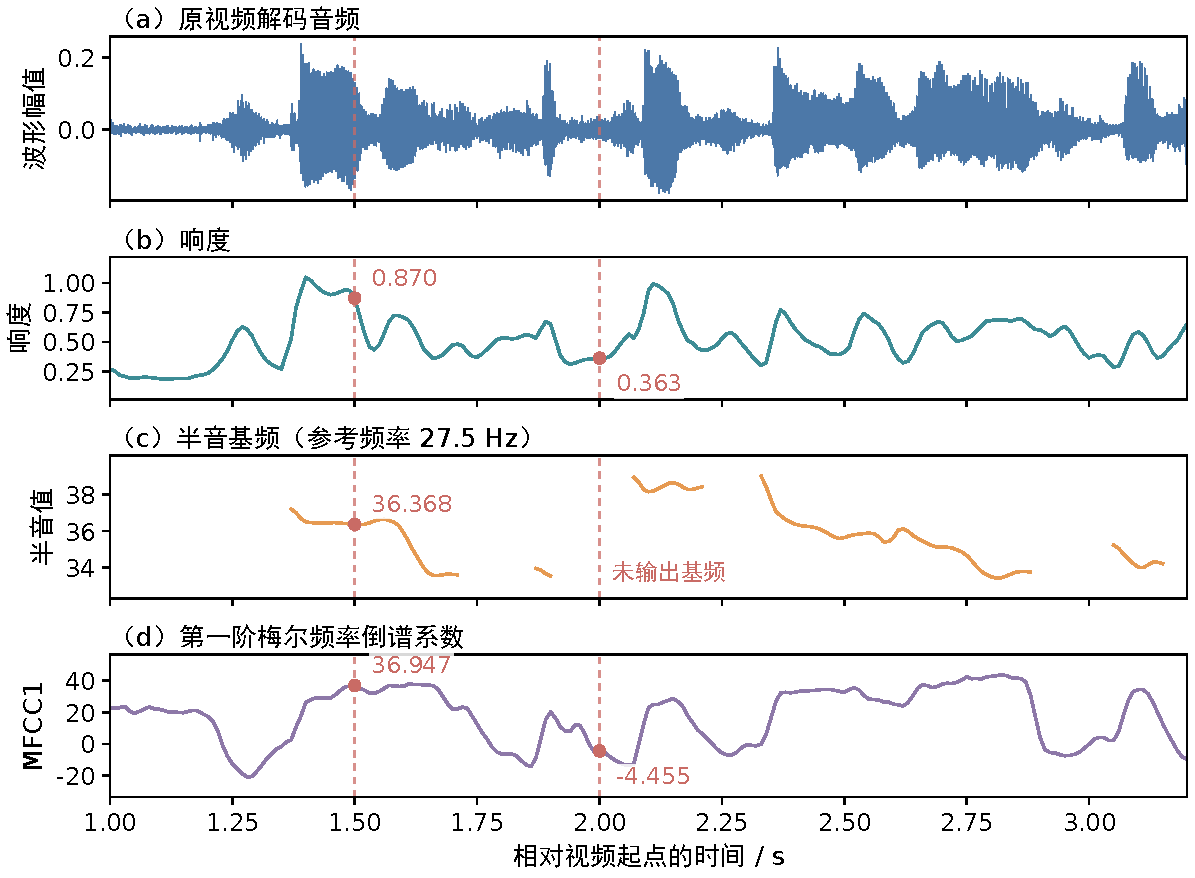
\includegraphics[width=\textwidth]{figures/fig_5_3_acoustic_example.pdf}
    \caption{同一语音片段的波形与声学特征。虚线标出记录中心为1.50 s和2.00 s的两组观测；各纵轴保留对应描述量的原始标度，不直接比较不同曲线的数值大小。}
    \label{fig:p1_acoustic_example}
\end{figure}

表~\ref{tab:p1_acoustic_example}列出了图中两组观测的具体数值。两条记录均具有有效音频观测，但第二条没有基频输出，说明声学记录的有效性与某一描述量是否得到估计应分别判断。该区间的响度和MFCC仍提供可用声学信息；MFCC的负值属于正常的投影结果，不能解释为能量为负。

\begin{table}[htbp]
    \centering
    \caption{两组声学观测的数值与有效性对照}
    \label{tab:p1_acoustic_example}
    \begingroup
    \small
    \setlength{\tabcolsep}{4pt}
    \renewcommand{\arraystretch}{1.2}
    \begin{tabular}{cccccc}
        \hline
        记录区间/s & 中心时刻/s & 响度 & 半音基频 & MFCC1 & 记录有效\\ \hline
        $[1.49,1.51]$ & 1.50 & 0.870 & 36.368 & 36.947 & 是\\
        $[1.99,2.01]$ & 2.00 & 0.363 & $0^{\ast}$ & $-4.455$ & 是\\ \hline
    \end{tabular}
    \par\smallskip
    \parbox{0.95\linewidth}{\footnotesize 注：$0^{\ast}$表示未输出有声基频时保留的零标记，不作为实际音高解释。响度与MFCC1沿用工具输出标度，半音基频以27.5 Hz为参考。}
    \endgroup
\end{table}

为使局部声学观测进一步参与词级对齐，按输出顺序保存各时刻的25维向量。设第$m$个声学向量为$\boldsymbol a_m\in\mathbb R^{25}$，共有$N_a$条记录，则原生声学特征矩阵为
\begin{equation}
    A=\begin{bmatrix}
        \boldsymbol a_1^{\mathsf T}\\
        \boldsymbol a_2^{\mathsf T}\\
        \vdots\\
        \boldsymbol a_{N_a}^{\mathsf T}
    \end{bmatrix}\in\mathbb R^{N_a\times25}.
    \label{eq:p1_audio_features}
\end{equation}
每行特征另关联工具返回的起止时间与观测有效标记，时间和标记均不计入25维特征。输出时间区间用于组织特征记录，而不同描述量内部采用的分析窗长并不相同，部分描述量还经过时间平滑。因此，后续将返回区间作为声学记录的时间支持近似，而不将其解释为所有描述量共同依赖的完整波形范围。

此时，矩阵$A$的每行对应一条声学记录，尚未与文本中的词一一对应。在后续词级时序对齐阶段，本文将根据候选词区间与声学记录区间的时间交叠关系进行加权聚合，形成与词级文本特征对应的声学表示。
